\documentclass{beamer}

\usetheme{Boadilla}

\title{Epidemic Broadcast}
\subtitle{Performance Evaluation of Computer Systems and Networks}
\author[Abdulwahed, Cima, Scatena]{Ahmed Khalil A. Abdulwahed, Lorenzo Cima, Niccolò Scatena}
\institute[UNIPI]{University of Pisa}
\date{2020/2021}

\begin{document}

\begin{frame}
	\titlepage{}
\end{frame}

\begin{frame}
	\frametitle{Outline}
	\tableofcontents
	TODO\@: remove this slide
\end{frame}

\section{Simulation model}

\begin{frame}
	\frametitle{The model}
	\begin{columns}
		\column{0.5\textwidth}
		\begin{itemize}
			\item 2D floorplan with users randomly dropped in
			\item A random user sends out a message; the other users
				relay it with a broadcast radius \emph{R}
			\item Time is \emph{slotted}
			\item \textbf{Trickle relaying}: when a user receives a
				message, it waits for \(T\) slots: message
				relayed if less than \(m\) copies received
		\end{itemize}
		\column{0.5\textwidth}
		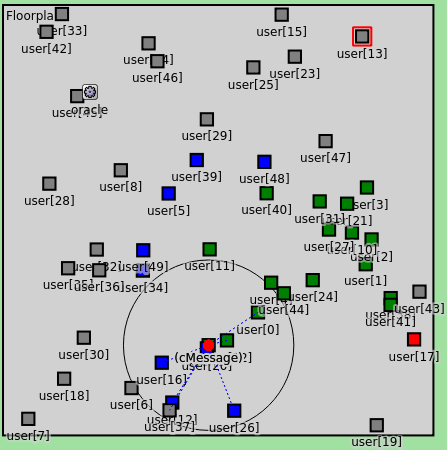
\includegraphics[width=\textwidth]{img/snapshot}
	\end{columns}
	Modules:
	\begin{description}
		\item[Floorplan] the network representing the 2D
			floorplan
		\item[User] submodule representing a user
		\item[Oracle] used to terminate simulation and collect
			some stats
	\end{description}
\end{frame}

\begin{frame}
	\frametitle{User module}
	\begin{columns}
		\column{0.5\textwidth}
		Finite State Machine
		\begin{description}
			\item[IDLE] state when started; slotting through
				self-messages
			\item[RECEIVING] hearing message in current slot
			\item[COLLISION] received another message in the same
				slot
			\item[HEARING] waiting for time window \(T\)
			\item[RELAYING] relay message if trickle relaying not
				triggered
		\end{description}
		\column{0.5\textwidth}
		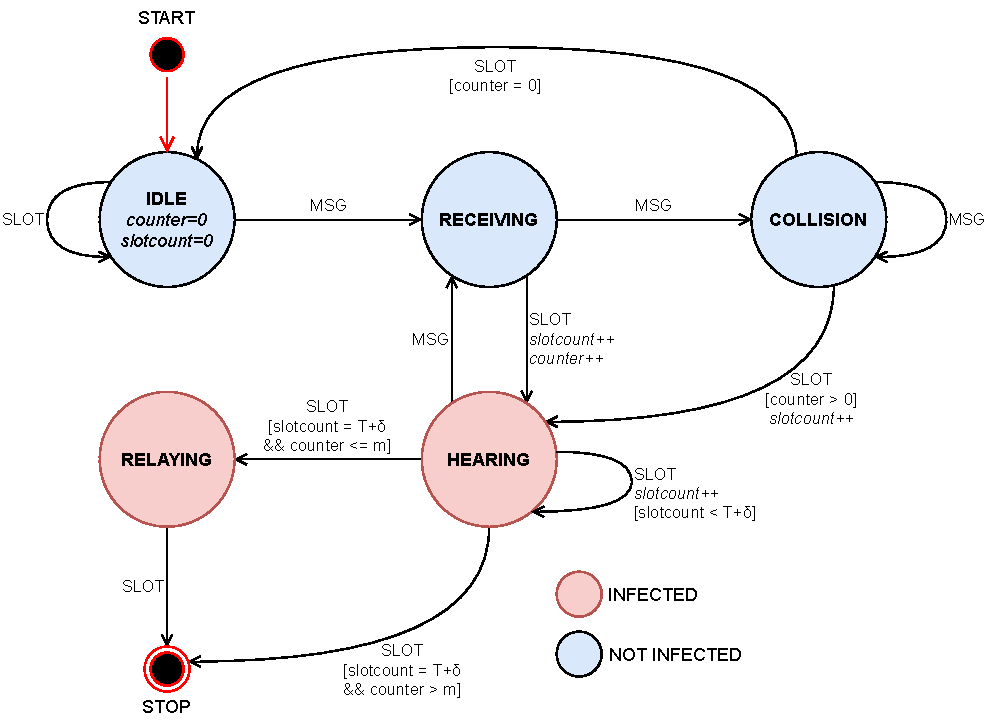
\includegraphics[width=\textwidth]{img/userfsm}
	\end{columns}
	User messages are sent with a duration equal to
	\(\frac{slotDuration}{2}\) in order to ensure that it is
	received in current slot
\end{frame}

\begin{frame}
	\frametitle{Model verification}
	\begin{columns}
		\column{0.5\textwidth}
		\begin{description}
			\item[Valgrind] no memory leaks
			\item[Graphical] execution inside QTEnv
			\item[Step-by-Step Debug] code execution path
			\item[Event Trace] check for correct scheduling
			\item[Deterministic] same inputs \textrightarrow{} same outputs
			\item[Degeneracy] config with low params values
			\item[Continuity] input change \textrightarrow{} output
				change (figure)
		\end{description}
		\column{0.5\textwidth}
		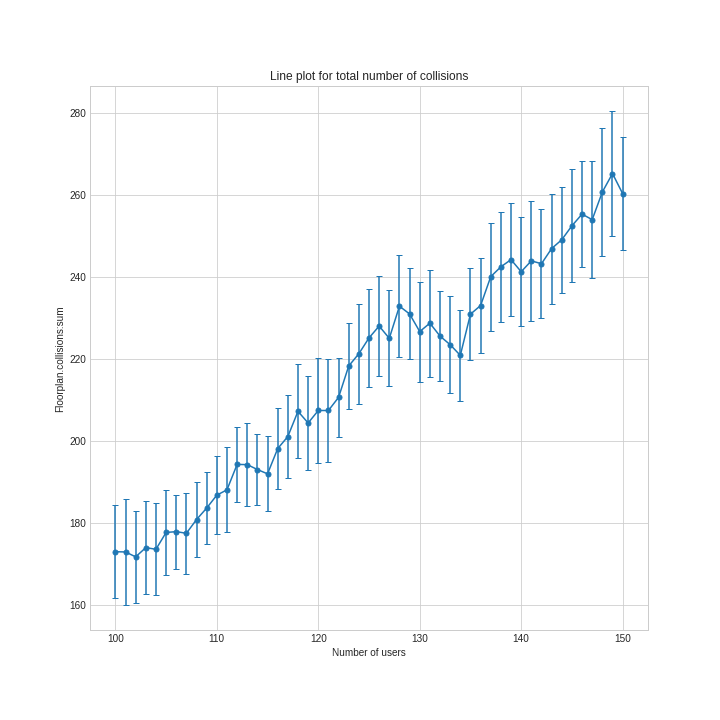
\includegraphics[width=\textwidth]{img/continuity-collisions}
	\end{columns}
\end{frame}

\section{Experiments design}

\begin{frame}
	\frametitle{Factors and Indexes}
	\begin{columns}
		\column{0.5\textwidth}
		Performance indexes:
		\begin{itemize}
			\item \textbf{Broadcast time} needed to cover a certain
				percentile of the users
			\item Final percentage of \textbf{covered users}
			\item \textbf{Energy efficiency}: depends on \(R\) and
				the number of messages sent
				\[\mathit{Eff} \propto \frac{1}{R \cdot M}\]
			\item \textbf{Collisions}
		\end{itemize}
		\column{0.5\textwidth}
		Tunable factors:
		\begin{itemize}
			\item Broadcast radius (\(R\))
			\item Trickle relaying hear window (\(T\))
			\item Trickle relaying max copies (\(m\))
			\item Maximum relay delay (\(\max(\delta)\)): introduced
				to avoid an issue with trickle relaying
		\end{itemize}
		Not tunable factors:
		\begin{itemize}
			\item Floorplan area (\(A\)) and dimensions ratio
				(\(\frac{X}{Y}\))
			\item User density (\(\frac{N}{A}\))
			\item Position of first user sending the message
		\end{itemize}
	\end{columns}
\end{frame}

\begin{frame}
	\frametitle{Scenarios}
	\begin{columns}
		\column{0.65\textwidth}
		\begin{description}
			\item[High Density] \(A = 22500m^2\) (\(150m \times
				150m\)), \(N = 1125\mathit{users}\) (\(0.05
					\mathit{users}/m^2\))
			\item[Low Density] \(A = 250000m^2\) (\(500m \times
				500m\)), \(N = 1250\mathit{users}\) (\(0.005
					\mathit{users}/m^2\))
			\item[Rectangular] \(A = 30000m^2\) (\(300m \times
				100m\)), \(N = 1500\mathit{users}\) (\(0.05
					\mathit{users}/m^2\))
		\end{description}
		\column{0.35\textwidth}
		\begin{itemize}
			\item \(T \in [5s, 10s]\)
			\item \(\max(\delta) \in [5s, 10s]\)
			\item \(m \in [2, 6]\)
			\item \(R \in [30m, 50m]\) (low density)\\
				\(R \in [10m, 20m]\) (others)
		\end{itemize}
	\end{columns}
	\begin{block}{Analysis workflow}
		\(2^{k}r\) to spot most important factors for each index. Then
		in-depth factorial analysis with the most important factors to
		study the behaviour between extreme values.
	\end{block}
	Jupyter notebooks: analysis automation
\end{frame}

\section{Analysis}

\begin{frame}
	\frametitle{High density}
	Probably each scenario requires 2 slides
\end{frame}

\begin{frame}
	\frametitle{Low density}
\end{frame}

\begin{frame}
	\frametitle{Rectangular floorplan}
\end{frame}

\begin{frame}
	\frametitle{Position of starting node}
\end{frame}

\section{Conclusions}
\begin{frame}
	\frametitle{Conclusions}
\end{frame}

\section{Some Stuff}

\begin{frame}
	\frametitle{Lists}
	\begin{enumerate}
		\item Point A
		\item Point B
		\begin{description}
			\item[Something] This is something
			\item[Foo] This is foo
		\end{description}
		\item Point C
		\begin{itemize}
			\item First item
			\item Second item
		\end{itemize}
		\item Point D
	\end{enumerate}
\end{frame}

\begin{frame}
	\frametitle{Columns, Tables, Images}
	\begin{columns}
		\column{0.5\textwidth}
		This is some text.

		Second line of left text.

		\begin{table}
			\begin{tabular}{l | c | c}
				First column & Second & Third \\
				\hline \hline
				Something & 110 & 123 \\
				Second Row & abc & def
			\end{tabular}
			\caption{Some data}
		\end{table}
		\column{0.5\textwidth}
		An image.

		
\includegraphics[scale=0.2]{img/marchio_unipi_pant541}
	\end{columns}
\end{frame}

\section{Blocks}

\begin{frame}
	\frametitle{Basic Blocks}
	\begin{block}{Block Title}
		Lorem ipsum dolor sit amet, consectetur adipisicing elit, sed do
		eiusmod tempor incididunt ut labore et	dolore magna aliqua.
	\end{block}
	\begin{alertblock}{Alert Title}
		Lorem ipsum dolor sit amet, consectetur adipisicing elit, sed do
		eiusmod tempor incididunt ut labore et	dolore magna aliqua.
	\end{alertblock}
	\begin{definition}
		Lorem ipsum dolor sit amet, consectetur adipisicing elit, sed do
		eiusmod tempor incididunt ut labore et	dolore magna aliqua.
	\end{definition}
	\begin{example}
		Lorem ipsum dolor sit amet, consectetur adipisicing elit, sed do
		eiusmod tempor incididunt ut labore et	dolore magna aliqua.
	\end{example}
\end{frame}

\subsection{Other Blocks}

\begin{frame}
	\frametitle{Math Blocks}
	\begin{theorem}{Pythagora}
		\( a^2 + b^2 = c^2 \)
	\end{theorem}
	\begin{corollary}
		\( x + y = y + x \)
	\end{corollary}
	\begin{proof}
		\( \omega + \phi = \epsilon \)

		\( \alpha + \beta = \frac{5}{7} \)
	\end{proof}
\end{frame}

\begin{frame}[fragile]
	\frametitle{Code Blocks}
	\begin{semiverbatim}
		#include <stdio.h>

		int main ()
		\{
			printf("Hello World!\\n");
			return 0;
		\}
	\end{semiverbatim}
\end{frame}

\section{Animations}

\subsection{Pause}

\begin{frame}
	\frametitle{Pause}
	\begin{itemize}
		\pause{}
		\item Point A
		\pause{}
		\item Point B
		\begin{itemize}
			\pause{}
			\item part 1
			\pause{}
			\item part 2
		\end{itemize}
		\pause{}
		\item Point C
			\pause{}
		\item Point D
	\end{itemize}
\end{frame}

\subsection{Overlays}

\begin{frame}
	\frametitle{Overlays}
	\textbf<2>{Example Text}\\
	\textit<2>{Example Text}\\
	\textsl<2>{Example Text}\\
	\textrm<2>{Example Text}\\
	\textsf<2>{Example Text}\\
	\textcolor<2>{orange}{Example Text}\\
	\alert<2>{Example Text}\\
	\structure<2>{Example Text}
\end{frame}

\begin{frame}
	\frametitle{Overlays (invisible)}
	\onslide<1->{First Line of Text}

	\onslide<2->{Second Line of Text}

	\onslide<3->{Third Line of Text}
\end{frame}

\setbeamercovered{transparent}

\begin{frame}
	\frametitle{Overlays (transparent)}
	\onslide<1->{First Line of Text}

	\onslide<2->{Second Line of Text}

	\onslide<3->{Third Line of Text}

\end{frame}

\setbeamercovered{invisible}

\end{document}
